\section{CircuitLab}

%%%%%%%%%%%%%%%%%%%%%%%%%%%%%%%%%%%%%%%
\subsection*{Hotkeys}
\begin{tabular}{l l l}
Action &    Shortcut  &     Mac \\ \hline
Save &     Ctrl+S &     \cmd +S \\
Save As &     Ctrl+Shift+S &     \cmd +Shift+S \\
Undo &     Ctrl+Z &     \cmd +Z \\
Delete &     Del &     Del \\
Cut &     Ctrl+X &     \cmd +X \\
Copy &     Ctrl+C &     \cmd +C \\
Paste &     Ctrl+V &     \cmd +V \\
Rotate C &     R &     R \\
Rotate CC &     Shift+R &     Shift+R \\
Flip Horiz. &     H &     H \\
Flip Vert. &     V &     V \\ 
Zoom In &     Ctrl + &     \cmd  + \\ 
Zoom Out &     Ctrl - &     \cmd  - \\
Select All &     Ctrl+A &     \cmd +A \\
Select None &     Ctrl+Shift+A &     \cmd +Shift+A \\
Pan &     Ctrl+<drag> & \cmd +<drag> \\
Build-mode &     Dbl-click &     Dbl-click \\
Simulate &     F5 &     F5 \\
$\neg$ smart wire &     Alt &     Alt \\
\end{tabular}



%%%%%%%%%%%%%%%%%%%%%%%%%%%%%%%%%%%%%%%
\subsection*{Expressions}
\textit{Where I(node,term), V(node), P(elem), PH(z$\in \mathbb{C}$) for current, voltage, power, phase; and PW[L|S][REPEAT]? for piecewise fn\textquotesingle s of time.}\\
\begin{tabular}{l l l l}
+    & -   & * & /  \\
\textasciicircum    & <  & > & ABS  \\ 
ACOS    & ACOSH  & ASIN  & ASINH  \\
ATAN    & ATANH  & CONJ  &  \\ 
COS    & COSH  & SIN  & SINH  \\
DB    & EXP  & I  & IF  \\ 
IMAG    & LIMIT  & LN  & LOG  \\
MAG    & MAX  & MIN  & P  \\ 
PH    & PHDEG  & PWL  & PWS  \\ 
REAL    & SQRT  & TAN  & TANH  \\ 
UNITLESS    & URAMP  & USTEP  & V  \\ 
\end{tabular}


%%%%%%%%%%%%%%%%%%%%%%%%%%%%%%%%%%%%%%%
\subsection*{Idioms}
\textit{Use labels ($\neg$ wires) to connect common signals:}
\resizebox{!}{2cm}{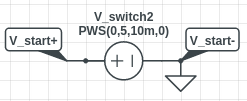
\includegraphics[]{images/CL-labels.png}}\\
\textit{Voltage-controlled switching for steps:}\\
\resizebox{!}{2cm}{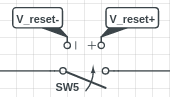
\includegraphics[]{images/CL-VCswitch.png}}

